\chapter{TÍNH TOÁN, THIẾT KẾ HỆ THỐNG ĐIỆN}
    \section{Thiết kế sơ đồ nguyên lý điện}
        \begin{figure}[H]
            \centering
            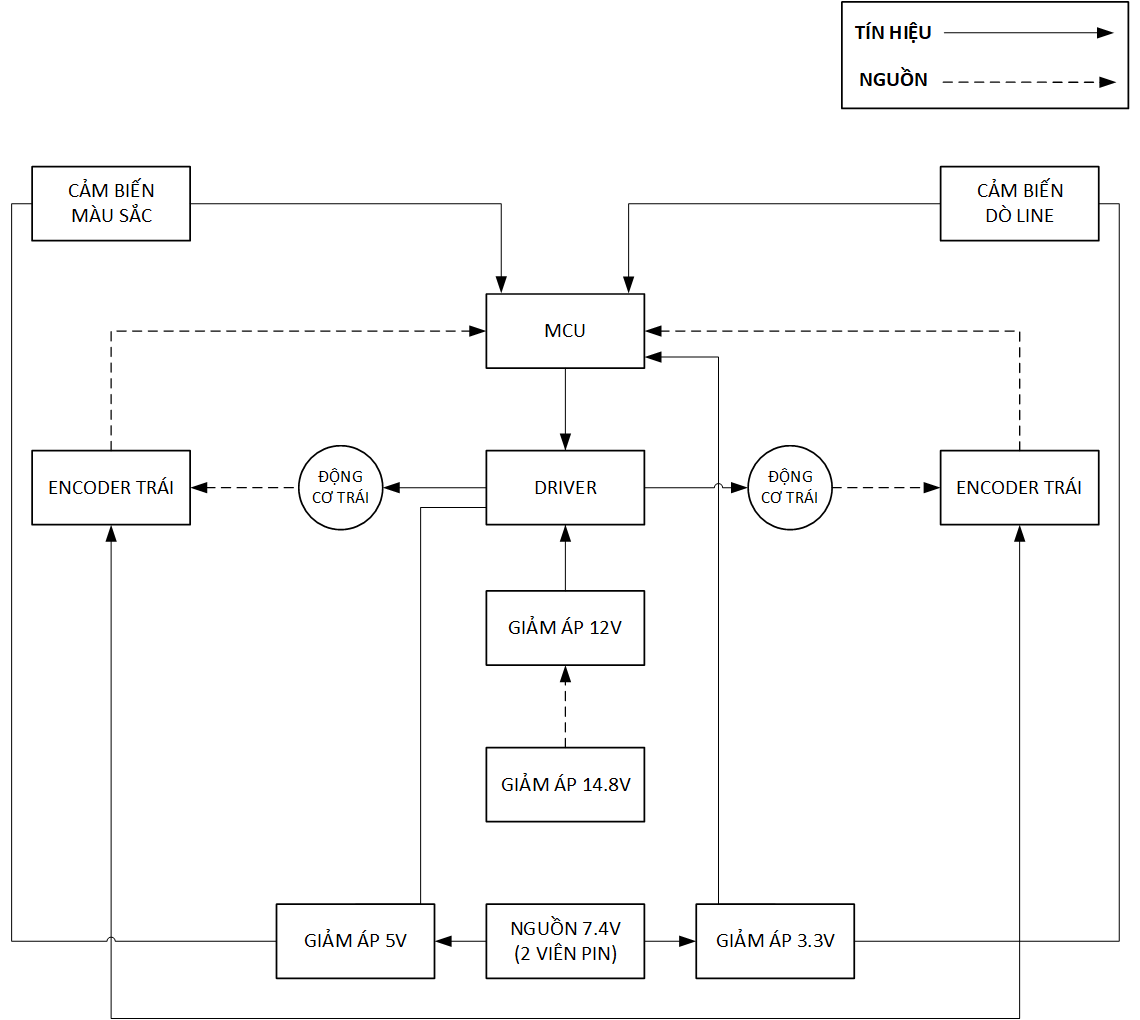
\includegraphics[width=1\textwidth]{pictures/chapter4/c4_p1_ElectricalFlow.png}
            \caption{Sơ đồ nguyên lý điện của hệ thống}
            \label{fig:4-1}
        \end{figure}
    \section{Thiết kế mạch cảm biến}
        \subsection{Tính chọn điện trở cho cảm biến dò line}
            \hspace*{0.6cm}Theo datasheet, ta có các thông số của TCRT5000 như sau:
            \begin{itemize}
                \item Khoảng cách hoạt động 12 (mm)
                \item Góc phát: $ 16^{\circ}$
                \item Góc thu: $ 30^{\circ}$
                \item Dòng lớn nhất qua phototransistor: $ I_{C} = 100$ (mA)
                \item Dòng lớn nhất qua LED: $I_{F} \leq 60$ (mA)
                \item Điện áp giữa A và K: $V_{AK} = 1.25$ (V)
            \end{itemize}
            \begin{figure}[H]
                \centering
                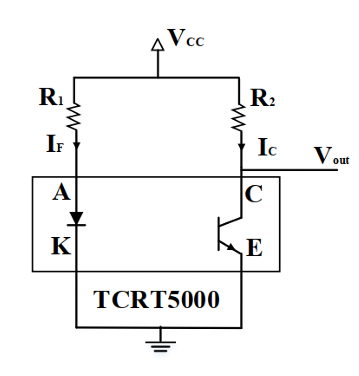
\includegraphics[width=0.35\textwidth]{pictures/chapter4/c4_p2_TCRT5000Schematic.png}
                \caption{Sơ đồ mạch điện TCRT5000}
                \label{fig:4-2}
            \end{figure}
            \hspace*{0.6cm}Dựa vào đường đặc tuyến trên datasheet, ta chọn $V_{F} = 1.1$ (V) và $I_{F} = 10$ (mA).\\
            \begin{figure}[H]
                \centering
                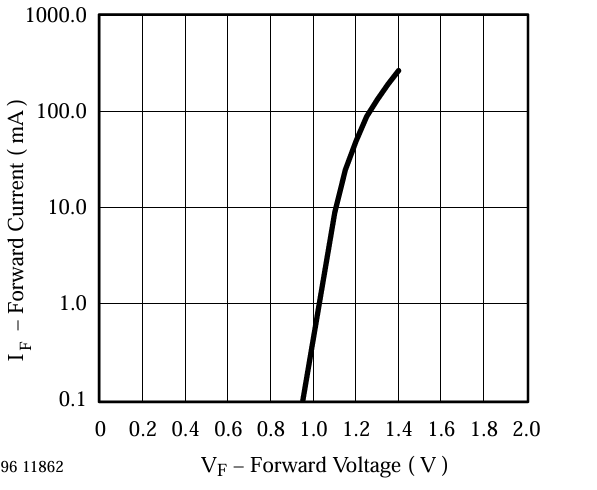
\includegraphics[width=0.5\textwidth]{pictures/chapter4/c4_p3_Voltage&Current.png}
                \caption{Đường đặc tuyến $V_{F}$ và $I_{F}$ của TCRT5000}
                \label{fig:4-3}
            \end{figure}
            Để tính điện trở R1, ta sử dụng công thức:
            \begin{equation}
                R_{1} = \frac{V_{CC} - V_{AK}}{I_{F}} = \frac{3.3 - 1.1}{0.01} = 220 \Omega
                \label{eq:4-1}
            \end{equation}
            \hspace*{0.6cm}Chọn điện trở R1 là $220 \Omega$ theo tiêu chuẩn trên thị trường.\\[0.4cm]
            \hspace*{0.6cm}Từ đường đặc tuyến $I_{C} - I_{F}$. Với $I_{F} = 10$ (mA) $\Rightarrow$ $I_{C} \approx 1$ (mA).
            \begin{figure}[H]
                \centering
                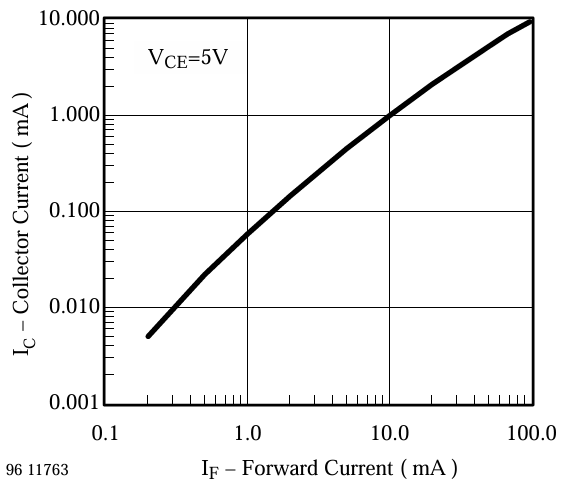
\includegraphics[width=0.5\textwidth]{pictures/chapter4/c4_p4_IC&IF.png}
                \caption{Đường đặc tuyến $I_{C}$ và $I_{F}$ của TCRT5000}
                \label{fig:4-4}
            \end{figure}
            Từ đường đặc tuyến $V_{CE} - I_{C} - I_{F}$, với $I_{C} = 1$ (mA) và $I_{F} = 10$ (mA) $\Rightarrow$ $V_{CE} \approx 1$ (V).\\
            \begin{figure}[H]
                \centering
                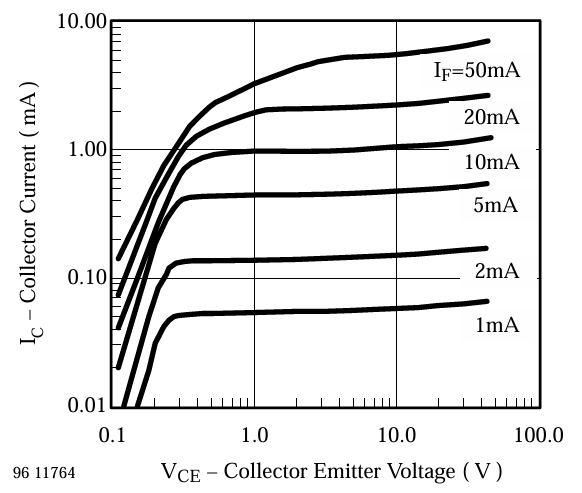
\includegraphics[width=0.5\textwidth]{pictures/chapter4/c4_p5_VCE&IC&IF.png}
                \caption{Đường đặc tuyến $V_{CE}$, $I_{C}$ và $I_{F}$ của TCRT5000}
                \label{fig:4-5}
            \end{figure}
            Từ đó, ta tính điện trở R2:
            \begin{equation}
                R_{2} = \frac{V_{CC} - V_{CE}}{I_{C}} = \frac{3.3 - 1}{0.001} = 2300 \Omega
                \label{eq:4-2}
            \end{equation}
            \hspace*{0.6cm}Chọn điện trở R2 là $2.4 k\Omega$ theo tiêu chuẩn trên thị trường.\\[0.4cm]
        \subsection{Xác định cách đặt cảm biến}
            \hspace*{0.6cm}Có 2 cách đặt cảm biến dò line:
            \begin{itemize}
                \item Trục giữa của bộ phát (S) và thu (E) vuông góc với biên phân cách sáng – tối (Position 1).
                \item Trục giữa của bộ phát (S) và thu (E) song song với biên phân cách sáng – tối (Position 2).
            \end{itemize}
            \begin{figure}[H]
                \centering
                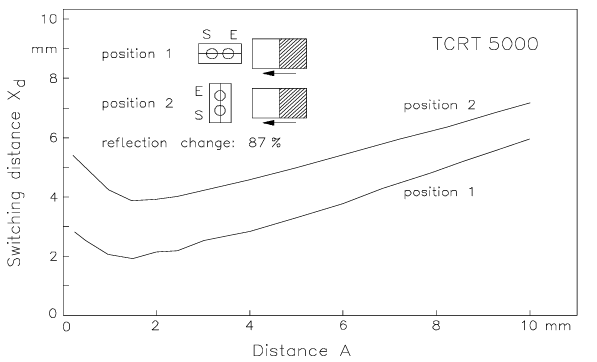
\includegraphics[width=0.8\textwidth]{pictures/chapter4/c4_p6_SensorPosition.png}
                \caption{So sánh độ phân giải của cảm biến khi đặt ở 2 vị trí khác nhau}
                \label{fig:4-5}
            \end{figure}
            \hspace*{0.6cm}Từ hình trên, ta thấy vị trí đặt cảm biến như Position 1 sẽ cho độ phân giải cao hơn so với Position 2. Do đó, ta chọn cách đặt cảm biến ở Position 1.
        \subsection{Xác định khoảng cách giữa các cảm biến}
            \begin{figure}[H]
                \centering
                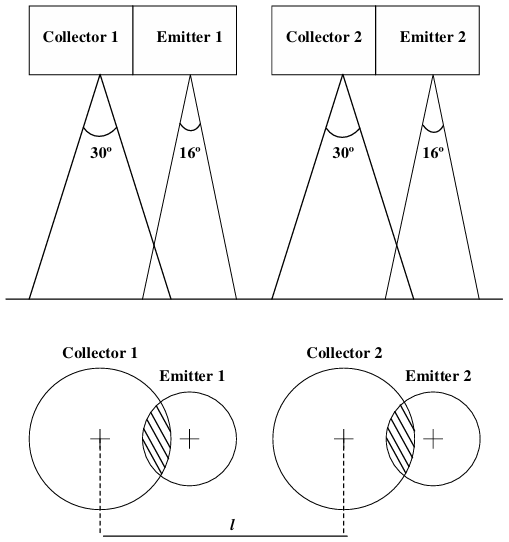
\includegraphics[width=0.7\textwidth]{pictures/chapter4/c4_p7_DistanceCollectorEmitter.png}
                \caption{Khoảng cách giữa các vùng thu và vùng phát}
                \label{fig:4-6}
            \end{figure}
            

            